
% -- classes do documento --
\documentclass[
	% -- classe de construcao --
		12pt, % tamanho da fonte
		%openright % capitulos começam em pag impar (insere pag vazia caso preciso)
		oneside, % impressao em apenas um lado
		a4paper, % formato do papel: A4
		article, % classe do documento: Artigo
	% -- opcoes da classe abntex2 --
		chapter=TITLE, % titulos de capitulos convertidos em letras maiusculas
		section=TITLE, % titulos de secoes convertidos em letras maiusculas
		subsection=TITLE, % titulos de subsecoes convertidos em letras maiusculas
	% -- opções do pacote babel --
		english, % idioma adicional para hifenizacao
		spanish, % idioma adicional para hifenizacao
		brazil % o ultimo idioma e o principal do documento
]{abntex2} % padrao ABNT2


% -- incusao de pacotes --
\usepackage[utf8]{inputenc} % codificacao do documento para leitura de caracteres unicode
\usepackage[brazil]{babel} % interpretacao do idioma pt-br
\usepackage{lmodern} % fonte Latin Modern
\usepackage{indentfirst} % indenta o primeiro paragrafo de cada secao
\usepackage{microtype} % para melhorias de justificação
\usepackage{color} % controle das cores
\usepackage[T1]{fontenc} % selecao de codigos de fonte
\usepackage{minted} % destaque de cores para codigos
\usepackage{amsmath, amsfonts, calc, xcolor} % inclusao de formulas matematicas
\usepackage{graphicx} % inclusao de graficos e imagens
\usepackage{hyperref} % referencia a conteudos do arquivo
\usepackage[brazilian, hyperpageref]{backref} % paginas de citacoes na bibl
\usepackage[alf, abnt-etal-list=0, abnt-etal-cite=1]{abntex2cite} % citacoes padrao ABNT
\usepackage{lipsum} % geracao de texto Lorem Ipsum
\usepackage{lastpage} % usado pela ficha catalografica


% -- configuracoes de estilos de capitulos e outras configuracoes --
\numberwithin{equation}{section}
\numberwithin{figure}{section}
\numberwithin{table}{section}
\linespread{0.95}

\makeatletter
	\setlength{\@fptop}{5pt} % posicionar figuras e tabelas no topo da pag quando adicionadas sozinhas em um pag em branco
\makeatother

\renewcommand{\ABNTEXpartfontsize}{\normalsize}
\renewcommand{\ABNTEXchapterfontsize}{\normalsize}
\renewcommand{\ABNTEXsectionfontsize}{\normalsize}
\renewcommand{\ABNTEXsubsectionfontsize}{\normalsize}

\renewcommand{\familydefault}{\sfdefault}
\renewcommand{\rmdefault}{phv}
\renewcommand{\sfdefault}{phv}
\renewcommand{\ttdefault}{pcr}

\renewcommand{\backrefpagesname}{Citado na(s) página(s):~}
\renewcommand{\backref}{}
\renewcommand*{\backrefalt}[4]{
	\ifcase #1
		Nenhuma citação no texto.
	\or
		Citado na página #2.
	\else
		Citado #1 vezes nas páginas #2.
	\fi
}

\newcommand{\quadroname}{Quadro}
\newcommand{\listofquadrosname}{Lista de quadros}

%\newfloat[chapter]{quadro}{loq}{\quadroname}
\newlistof{listofquadros}{loq}{\listofquadrosname}
\newlistentry{quadro}{loq}{0}

\setfloatadjustment{quadro}{\centering}
\counterwithout{quadro}{chapter}
\renewcommand{\cftquadroname}{\quadroname\space} 
\renewcommand*{\cftquadroaftersnum}{\hfill--\hfill}

\setfloatlocations{quadro}{hbtp}

% -- espacamento entre linhas e paragrafos --
\setlength{\parindent}{1.3cm}
\setlength{\parskip}{0.2cm}

% -- compila o indice --
\makeindex


% -- informacoes da capa e folha de rosto --
\titulo{Circuitos Resistivos em Série e Paralelo}
\autor{Álvaro Davi S. Alves}
\local{Goiabeiras - Vitória - ES - Brasil}
\data{2021, junho}
\orientador{Anselmo F. Neto}
\coorientador{Ricardo C. de Mello}
\instituicao{
	Universidade Federal do Espírito Santo
	\par
	Curso de Engenharia da Computação
}

\tipotrabalho{Exercício 02 de Práticas de Laboratório}
\preambulo{Resolução - Ex02: Circuitos Resistivos em Série e Paralelo}


% -- configuracoes do PDF --
\definecolor{blue}{RGB}{41, 5, 195}
\makeatletter
	\hypersetup{
		%pagebackref=true,
		pdftitle={\@title}, 
		pdfauthor={\@author},
		pdfcreator={Álvaro Davi Santos Alves},
		pdfkeywords={abnt}{latex}{abntex}{abntex2}{trabalho acadêmico}, 
		colorlinks=true, % links coloridos
		linkcolor=blue, % cor de links internos
		citecolor=blue, % cor de citacoes bibliograficas
		filecolor=magenta,
		urlcolor=blue,
		bookmarksdepth=4
	}
\makeatother


% -- inicio do documento --
\begin{document}
	\selectlanguage{brazil}

	\frenchspacing % retirar espaço extra obsoleto entre as frases

	%\maketitle % criar o titulo
	\phantompart % adicionar espaco para sumario

	% ----------------------------------------------------------
	% ELEMENTOS PRE-TEXTUAIS
	% ----------------------------------------------------------

	\imprimircapa

	\imprimirfolhaderosto* % (o * indica que havera a ficha bibliografica)

	% ----------------------------------------------------------
	% ELEMENTOS TEXTUAIS
	% ----------------------------------------------------------
	\textual

	\chapter{Circuito Resistivo em Série}

	\flushleft
	Sendo a equação da tensão e a equação da potência: \\
	\center
	$U = R*i$ \\
	e \\
	$P = U*i$ \\
	\flushleft
	E, consequentemente: \\
	\center
	$i = \frac{U}{R}$ \\
	\flushleft
	Temos que, por estar em série: \\
	\center
	$R_{eq} = \sum_{i=1}^{n} R_i$ \\


	\flushleft
	\textbf{a)} Assim: $R_{eq} = 1800 + 560 = 2360$, ou seja, $R_{eq} = 2,36 k\Omega$.
	\linebreak

	\textbf{b)} \\
	$i_T = \frac{12}{2360} \approx 0,00508  \approx 5,08 mA$

	$U_{R1} = 0,00508 * 1800 = 9,15V$ \\
	$U_{R2} = 0,00508 * 560 = 2,85V$
	\linebreak

	\textbf{c)} \\
	As imagens referentes a esta questão podem ser encontradas clicando na referência: \\
	\ref{fig:figura1} - Tensão de C1 em série \\
	\ref{fig:figura2} - Corrente de C1 em série
	\linebreak

	\textbf{d)} \\
	Se $V = V_1 + V_2 + ... + V_n$ \\
	Então: $V_1 + V_2 + ... + V_n - V = 0$

	Assim: $9,15V + 2,85V - 12V = 0V$

	Como não há malhas em C1, não é possível calcular a soma das correntes nas malhas, a mesma corrente segue diretamente do terminal positivo para o terminal negativo da fonte, passando apenas pelos resistores.
	\linebreak

	\textbf{e)} \\
	$P_F = 12 * 0,00508 \approx 0,0609 W$

	$P_{R1} = 9,15 * 0,00508 \approx 0,0464 W$ \\
	$P_{R2} = 2,85 * 0,00508 \approx 0,0144 W$


	\newpage

	\chapter{Circuito Resistivo em Paralelo}

	\flushleft
	Sendo a equação da tensão e a equação da potência: \\
	\center
	$U = R*i$ \\
	e \\
	$P = U*i$ \\
	\flushleft
	E, consequentemente: \\
	\center
	$i = \frac{U}{R}$ \\
	\flushleft
	Temos que, por estar em paralelo: \\
	\center
	$\frac{1}{R_{eq}} = \sum_{i=1}^{n}  \frac{1}{R_i}$ \\


	\flushleft
	\textbf{a)} Assim: $\frac{1}{R_{eq}} = \frac{1}{1800} + \frac{1}{560} = \frac{1}{0,0023} = 427$, ou seja, $R_{eq} = 427 \Omega$.
	\linebreak

	\textbf{b)} \\
	$i_T = \frac{12}{427} \approx 0,0281 \approx 28,1 mA$

	$i_{R1} =  \frac{12}{1800} \approx 0,00667 \approx 6,67 mA$ \\
	$i_{R2} =   \frac{12}{560} \approx 0,0214 \approx 21,4 mA$

	$U_{R1} =  0,00667 * 1800 = 12V$ \\
	$U_{R2} =  0,0214 * 560 = 12V$
	\linebreak

	\textbf{c)} \\
	As imagens referentes a esta questão podem ser encontradas clicando na referência: \\
	\ref{fig:figura3} - Tensão de C2 em paralelo \\
	\ref{fig:figura4} - Corrente de C2 em paralelo
	\linebreak

	\textbf{d)} \\
	Se $i_T = i_1 + i_2 + ... + i_n$ \\
	Então: $i_1 + i_2 + ... + i_n - i = 0$

	Assim: $6,67mA + 21,4mA - 28,1mA = 0mA$

	Como nesse caso, C2 está em paralelo, a mesma tensão recairá sobre as malhas: \\
	Se $V = V_1 + V_2 + ... + V_n$ \\
	Então: $V_1 + V_2 + ... + V_n - V = 0$

	$M_1: 12V - 12V = 0V$ \\
	$M_2: 12V - 12V = 0V$
	\linebreak

	\textbf{e)} \\
	$P_F = 12 * 0,0281 \approx 0,3372 W$

	$P_{R1} = 12 * 0,0066 \approx 0,2568 W$ \\
	$P_{R2} = 12 * 0,0214 \approx 0,0792 W$


	\newpage

	\chapter{Figuras}
	\begin{figure}[h]
		\graphicspath{ {./esquematicos/} }

		\caption{Tensão de C1 em série}
		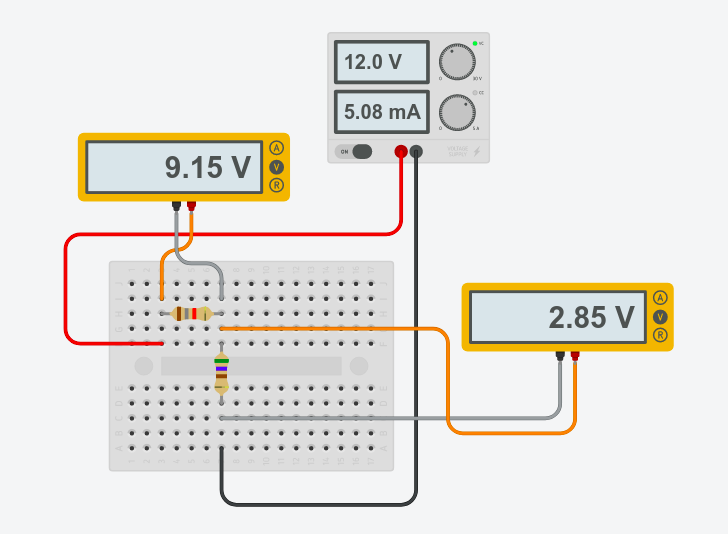
\includegraphics[width=15cm, height=14cm]{C1_S-T.png}
		\label{fig:figura1}

	\end{figure}
	\begin{figure}[h]
		\graphicspath{ {./esquematicos/} }

		\caption{Corrente de C1 em série}
		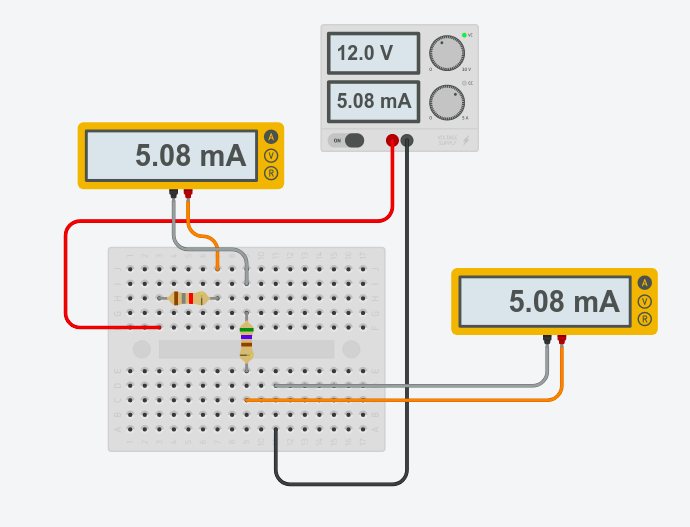
\includegraphics[width=15cm, height=14cm]{C1_S-C.png}
		\label{fig:figura2}

	\end{figure}
	\begin{figure}[h]
		\graphicspath{ {./esquematicos/} }

		\caption{Tensão de C2 em paralelo}
		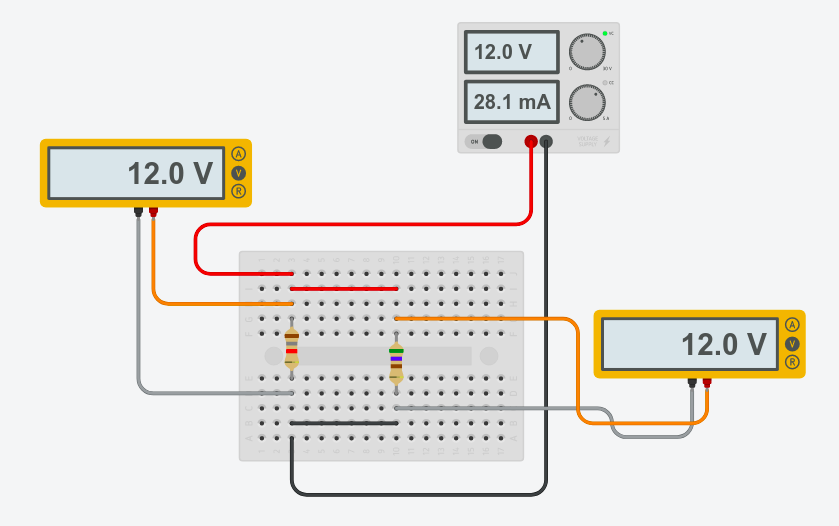
\includegraphics[width=15cm, height=14cm]{C2_P-T.png}
		\label{fig:figura3}

	\end{figure}
	\begin{figure}[h]
		\graphicspath{ {./esquematicos/} }

		\caption{Corrente de C2 em paralelo}
		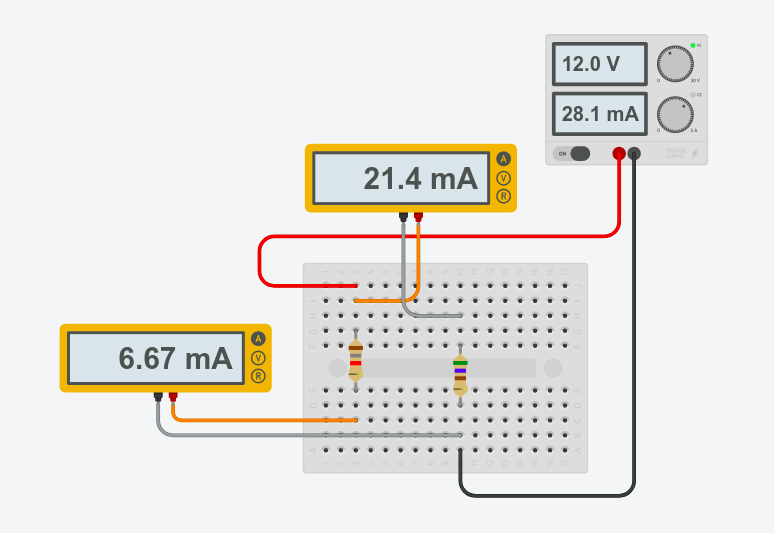
\includegraphics[width=15cm, height=14cm]{C2_P-C.png}
		\label{fig:figura4}

	\end{figure}



\end{document}
